\documentclass[nooutcomes]{ximera}


\graphicspath{
  {./}
  {1-1QuantitativeReasoning/}
  {1-2RelationsAndGraphs/}
  {1-3ChangingInTandem/}
  {2-1LinearEquations/}
  {2-2LinearModeling/}
  {2-3ExponentialModeling/}
  {3-1WhatIsAFunction/}
  {3-2FunctionProperties/}
  {3-3AverageRatesOfChange/}
  {4-1BuildingNewFunctions/}
  {4-2Polynomials/}
  {5-1RationalFunctions/}
   {5-2ExponentialFunctions/}
  {6-1Domain/}
  {6-2Range/}
  {6-3CompositionOfFunctions/}
  {7-1ZerosOfFunctions/}
  {7-XZerosOfPolynomials/}
  {7-2ZerosOfFamousFunctions/}
  {8-0Review/}
  {8-1FunctionTransformations/}
  {8-2SolvingInequalities/}
  {8-3FunctionTransformationsProject/}
  {9-1RightTriangleTrig/}
  {9-2TheUnitCircle/}
  {9-3TrigIdentities/}
  {10-1UnitCircleToFunctionGraph/}
  {10-2TrigFunctions/}
  {10-3SomeApplicationsOfTrig/}
  {11-1InverseFunctionsRevisited/}
  {11-2Logarithms/}
  {11-3InverseTrig/}
  {12-1SystemsOfEquations/}
  {12-2NonlinearSystems/}
  {12-3ApplicationsOfSystems/}
  {13-1SecantLinesRevisited/}
  {13-2Functions-TheBigPicture/}
  {14-1DisplacementVsDistance/}
  {1-1QuantitativeReasoning/exercises/}
  {1-2RelationsAndGraphs/exercises/}
  {../1-3ChangingInTandem/exercises/}
  {../2-1LinearEquations/exercises/}
  {../2-2LinearModeling/exercises/}
  {../2-3ExponentialModeling/exercises/}
  {../3-1WhatIsAFunction/exercises/}
  {../3-2FunctionProperties/exercises/}
  {../3-3AverageRatesOfChange/exercises/}
  {../5-2ExponentialFunctions/exercises/}
  {../4-1BuildingNewFunctions/exercises/}
  {../4-2Polynomials/exercises/}
  {../5-1RationalFunctions/exercises/}
  {../6-1Domain/exercises/}
  {../6-2Range/exercises/}
  {../6-3CompositionOfFunctions/exercises/}
  {../7-1ZerosOfFunctions/exercises/}
  {../7-XZerosOfPolynomials/exercises/}
  {../7-2ZerosOfFamousFunctions/exercises/}
  {../8-1FunctionTransformations/exercises/}
  {../12-1SystemsOfEquations/exercises/}
  {../8-3FunctionTransformationsProject/exercises/}
  {../8-0Review/exercises/}
  {../8-2SolvingInequalities/exercises/}
  {../8-3FunctionTransformationsProject/exercises/}
  {../9-1RightTriangleTrig/exercises/}
  {../9-2TheUnitCircle/exercises/}
  {../9-3TrigIdentities/exercises/}
  {../10-1UnitCircleToFunctionGraph/exercises/}
  {../10-2TrigFunctions/exercises/}
  {../10-3SomeApplicationsOfTrig/exercises/}
  {../11-1InverseFunctionsRevisited/exercises/}
  {../11-2Logarithms/exercises/}
  {../11-3InverseTrig/exercises/}
  {../12-1SystemsOfEquations/exercises/}
  {../12-2NonlinearSystems/exercises/}
  {../12-3ApplicationsOfSystems/exercises/}
  {../13-1SecantLinesRevisited/exercises/}
  {../13-2Functions-TheBigPicture/exercises/}
  {../14-1DisplacementVsDistance/exercises/}
}

\DeclareGraphicsExtensions{.pdf,.png,.jpg,.eps}

\newcommand{\mooculus}{\textsf{\textbf{MOOC}\textnormal{\textsf{ULUS}}}}

\usepackage[makeroom]{cancel} %% for strike outs

\ifxake
\else
\usepackage[most]{tcolorbox}
\fi


%\typeout{************************************************}
%\typeout{New Environments}
%\typeout{************************************************}

%% to fix for web can be removed when deployed offically with ximera2
\let\image\relax\let\endimage\relax
\NewEnviron{image}{% 
  \begin{center}\BODY\end{center}% center
}



\NewEnviron{folder}{
      \addcontentsline{toc}{section}{\textbf{\BODY}}
}

\ifxake
\let\summary\relax
\let\endsummary\relax
\newtheorem*{summary}{Summary}
\newtheorem*{callout}{Callout}
\newtheorem*{overview}{Overview}
\newtheorem*{objectives}{Objectives}
\newtheorem*{motivatingQuestions}{Motivating Questions}
\newtheorem*{MM}{Metacognitive Moment}
      
%% NEEDED FOR XIMERA 2
%\ximerizedEnvironment{summary}
%\ximerizedEnvironment{callout}
%\ximerizedEnvironment{overview} 
%\ximerizedEnvironment{objectives}
%\ximerizedEnvironment{motivatingQuestions}
%\ximerizedEnvironment{MM}
\else
%% CALLOUT
\NewEnviron{callout}{
  \begin{tcolorbox}[colback=blue!5, breakable,pad at break*=1mm]
      \BODY
  \end{tcolorbox}
}
%% MOTIVATING QUESTIONS
\NewEnviron{motivatingQuestions}{
  \begin{tcolorbox}[ breakable,pad at break*=1mm]
    \textbf{\Large Motivating Questions}\hfill
    %\begin{itemize}[label=\textbullet]
      \BODY
    %\end{itemize}
  \end{tcolorbox}
}
%% OBJECTIVES
\NewEnviron{objectives}{  
    \vspace{.5in}
      %\begin{tcolorbox}[colback=orange!5, breakable,pad at break*=1mm]
    \textbf{\Large Learning Objectives}
    \begin{itemize}[label=\textbullet]
      \BODY
    \end{itemize}
    %\end{tcolorbox}
}
%% DEFINITION
\let\definition\relax
\let\enddefinition\relax
\NewEnviron{definition}{
  \begin{tcolorbox}[ breakable,pad at break*=1mm]
    \noindent\textbf{Definition}~
      \BODY
  \end{tcolorbox}
}
%% OVERVIEW
\let\overview\relax
\let\overview\relax
\NewEnviron{overview}{
  \begin{tcolorbox}[ breakable,pad at break*=1mm]
    \textbf{\Large Overview}
    %\begin{itemize}[label=\textbullet] %% breaks Xake
      \BODY
    %\end{itemize}
  \end{tcolorbox}
}
%% SUMMARY
\let\summary\relax
\let\endsummary\relax
\NewEnviron{summary}{
  \begin{tcolorbox}[ breakable,pad at break*=1mm]
    \textbf{\Large Summary}
    %\begin{itemize}[label=\textbullet] %% breaks Xake
      \BODY
    %\end{itemize}
  \end{tcolorbox}
}
%% REMARK
\let\remark\relax
\let\endremark\relax
\NewEnviron{remark}{
  \begin{tcolorbox}[colback=green!5, breakable,pad at break*=1mm]
    \noindent\textbf{Remark}~
      \BODY
  \end{tcolorbox}
}
%% EXPLANATION
\let\explanation\relax
\let\endexplanation\relax
\NewEnviron{explanation}{
    \normalfont
    \noindent\textbf{Explanation}~
      \BODY
}
%% EXPLORATION
\let\exploration\relax
\let\endexploration\relax
\NewEnviron{exploration}{
  \begin{tcolorbox}[colback=yellow!10, breakable,pad at break*=1mm]
    \noindent\textbf{Exploration}~
      \BODY
  \end{tcolorbox}
}
%% METACOGNITIVE MOMENTS
\let\MM\relax
\let\endMM\relax
\NewEnviron{MM}{
  \begin{tcolorbox}[colback=pink!15, breakable,pad at break*=1mm]
    \noindent\textbf{Metacognitive Moment}~
      \BODY
  \end{tcolorbox}
}


\fi





%Notes on what envirnoment to use:  Example with Explanation in text; if they are supposed to answer- Problem; no answer - Exploration


%\typeout{************************************************}
%% Header and footers
%\typeout{************************************************}

\newcommand{\licenseAcknowledgement}{Licensed under Creative Commons 4.0}
\newcommand{\licenseAPC}{\renewcommand{\licenseAcknowledgement}{\textbf{Acknowledgements:} Active Prelude to Calculus (https://activecalculus.org/prelude) }}
\newcommand{\licenseSZ}{\renewcommand{\licenseAcknowledgement}{\textbf{Acknowledgements:} Stitz Zeager Open Source Mathematics (https://www.stitz-zeager.com/) }}
\newcommand{\licenseAPCSZ}{\renewcommand{\licenseAcknowledgement}{\textbf{Acknowledgements:} Active Prelude to Calculus (https://activecalculus.org/prelude) and Stitz Zeager Open Source Mathematics (https://www.stitz-zeager.com/) }}
\newcommand{\licenseORCCA}{\renewcommand{\licenseAcknowledgement}{\textbf{Acknowledgements:}Original source material, products with readable and accessible
math content, and other information freely available at pcc.edu/orcca.}}
\newcommand{\licenseY}{\renewcommand{\licenseAcknowledgement}{\textbf{Acknowledgements:} Yoshiwara Books (https://yoshiwarabooks.org/)}}
\newcommand{\licenseOS}{\renewcommand{\licenseAcknowledgement}{\textbf{Acknowledgements:} OpenStax College Algebra (https://openstax.org/details/books/college-algebra)}}
\newcommand{\licenseAPCSZCSCC}{\renewcommand{\licenseAcknowledgement}{\textbf{Acknowledgements:} Active Prelude to Calculus (https://activecalculus.org/prelude), Stitz Zeager Open Source Mathematics (https://www.stitz-zeager.com/), CSCC PreCalculus and Calculus texts (https://ximera.osu.edu/csccmathematics)}}

\ifxake\else %% do nothing on the website
\usepackage{fancyhdr}
\pagestyle{fancy}
\fancyhf{}
\fancyhead[R]{\sectionmark}
\fancyfoot[L]{\thepage}
\fancyfoot[C]{\licenseAcknowledgement}
\renewcommand{\headrulewidth}{0pt}
\renewcommand{\footrulewidth}{0pt}
\fi

%%%%%%%%%%%%%%%%



%\typeout{************************************************}
%\typeout{Table of Contents}
%\typeout{************************************************}


%% Edit this to change the font style
\newcommand{\sectionHeadStyle}{\sffamily\bfseries}


\makeatletter

%% part uses arabic numerals
\renewcommand*\thepart{\arabic{part}}


\ifxake\else
\renewcommand\chapterstyle{%
  \def\maketitle{%
    \addtocounter{titlenumber}{1}%
    \pagestyle{fancy}
    \phantomsection
    \addcontentsline{toc}{section}{\textbf{\thepart.\thetitlenumber\hspace{1em}\@title}}%
                    {\flushleft\small\sectionHeadStyle\@pretitle\par\vspace{-1.5em}}%
                    {\flushleft\LARGE\sectionHeadStyle\thepart.\thetitlenumber\hspace{1em}\@title \par }%
                    {\setcounter{problem}{0}\setcounter{sectiontitlenumber}{0}}%
                    \par}}





\renewcommand\sectionstyle{%
  \def\maketitle{%
    \addtocounter{sectiontitlenumber}{1}
    \pagestyle{fancy}
    \phantomsection
    \addcontentsline{toc}{subsection}{\thepart.\thetitlenumber.\thesectiontitlenumber\hspace{1em}\@title}%
    {\flushleft\small\sectionHeadStyle\@pretitle\par\vspace{-1.5em}}%
    {\flushleft\Large\sectionHeadStyle\thepart.\thetitlenumber.\thesectiontitlenumber\hspace{1em}\@title \par}%
    %{\setcounter{subsectiontitlenumber}{0}}%
    \par}}



\renewcommand\section{\@startsection{paragraph}{10}{\z@}%
                                     {-3.25ex\@plus -1ex \@minus -.2ex}%
                                     {1.5ex \@plus .2ex}%
                                     {\normalfont\large\sectionHeadStyle}}
\renewcommand\subsection{\@startsection{subparagraph}{10}{\z@}%
                                    {3.25ex \@plus1ex \@minus.2ex}%
                                    {-1em}%
                                    {\normalfont\normalsize\sectionHeadStyle}}

\fi

%% redefine Part
\renewcommand\part{%
   {\setcounter{titlenumber}{0}}
  \if@openright
    \cleardoublepage
  \else
    \clearpage
  \fi
  \thispagestyle{plain}%
  \if@twocolumn
    \onecolumn
    \@tempswatrue
  \else
    \@tempswafalse
  \fi
  \null\vfil
  \secdef\@part\@spart}

\def\@part[#1]#2{%
    \ifnum \c@secnumdepth >-2\relax
      \refstepcounter{part}%
      \addcontentsline{toc}{part}{\thepart\hspace{1em}#1}%
    \else
      \addcontentsline{toc}{part}{#1}%
    \fi
    \markboth{}{}%
    {\centering
     \interlinepenalty \@M
     \normalfont
     \ifnum \c@secnumdepth >-2\relax
       \huge\sffamily\bfseries \partname\nobreakspace\thepart
       \par
       \vskip 20\p@
     \fi
     \Huge \bfseries #2\par}%
    \@endpart}
\def\@spart#1{%
    {\centering
     \interlinepenalty \@M
     \normalfont
     \Huge \bfseries #1\par}%
    \@endpart}
\def\@endpart{\vfil\newpage
              \if@twoside
               \if@openright
                \null
                \thispagestyle{empty}%
                \newpage
               \fi
              \fi
              \if@tempswa
                \twocolumn
                \fi}



\makeatother





%\typeout{************************************************}
%\typeout{Stuff from Ximera}
%\typeout{************************************************}



\usepackage{array}  %% This is for typesetting long division
\setlength{\extrarowheight}{+.1cm}
\newdimen\digitwidth
\settowidth\digitwidth{9}
\def\divrule#1#2{
\noalign{\moveright#1\digitwidth
\vbox{\hrule width#2\digitwidth}}}





\newcommand{\RR}{\mathbb R}
\newcommand{\R}{\mathbb R}
\newcommand{\N}{\mathbb N}
\newcommand{\Z}{\mathbb Z}

\newcommand{\sagemath}{\textsf{SageMath}}


\def\d{\,d}
%\renewcommand{\d}{\mathop{}\!d}
\newcommand{\dd}[2][]{\frac{\d #1}{\d #2}}
\newcommand{\pp}[2][]{\frac{\partial #1}{\partial #2}}
\renewcommand{\l}{\ell}
\newcommand{\ddx}{\frac{d}{\d x}}



%\newcommand{\unit}{\,\mathrm}
\newcommand{\unit}{\mathop{}\!\mathrm}
\newcommand{\eval}[1]{\bigg[ #1 \bigg]}
\newcommand{\seq}[1]{\left( #1 \right)}
\renewcommand{\epsilon}{\varepsilon}
\renewcommand{\phi}{\varphi}


\renewcommand{\iff}{\Leftrightarrow}

\DeclareMathOperator{\arccot}{arccot}
\DeclareMathOperator{\arcsec}{arcsec}
\DeclareMathOperator{\arccsc}{arccsc}
\DeclareMathOperator{\sign}{sign}


%\DeclareMathOperator{\divergence}{divergence}
%\DeclareMathOperator{\curl}[1]{\grad\cross #1}
\newcommand{\lto}{\mathop{\longrightarrow\,}\limits}

\renewcommand{\bar}{\overline}

\colorlet{textColor}{black}
\colorlet{background}{white}
\colorlet{penColor}{blue!50!black} % Color of a curve in a plot
\colorlet{penColor2}{red!50!black}% Color of a curve in a plot
\colorlet{penColor3}{red!50!blue} % Color of a curve in a plot
\colorlet{penColor4}{green!50!black} % Color of a curve in a plot
\colorlet{penColor5}{orange!80!black} % Color of a curve in a plot
\colorlet{penColor6}{yellow!70!black} % Color of a curve in a plot
\colorlet{fill1}{penColor!20} % Color of fill in a plot
\colorlet{fill2}{penColor2!20} % Color of fill in a plot
\colorlet{fillp}{fill1} % Color of positive area
\colorlet{filln}{penColor2!20} % Color of negative area
\colorlet{fill3}{penColor3!20} % Fill
\colorlet{fill4}{penColor4!20} % Fill
\colorlet{fill5}{penColor5!20} % Fill
\colorlet{gridColor}{gray!50} % Color of grid in a plot

\newcommand{\surfaceColor}{violet}
\newcommand{\surfaceColorTwo}{redyellow}
\newcommand{\sliceColor}{greenyellow}




\pgfmathdeclarefunction{gauss}{2}{% gives gaussian
  \pgfmathparse{1/(#2*sqrt(2*pi))*exp(-((x-#1)^2)/(2*#2^2))}%
}





%\typeout{************************************************}
%\typeout{ORCCA Preamble.Tex}
%\typeout{************************************************}


%% \usepackage{geometry}
%% \geometry{letterpaper,total={408pt,9.0in}}
%% Custom Page Layout Adjustments (use latex.geometry)
%% \usepackage{amsmath,amssymb}
%% \usepackage{pgfplots}
\usepackage{pifont}                                         %needed for symbols, s.a. airplane symbol
\usetikzlibrary{positioning,fit,backgrounds}                %needed for nested diagrams
\usetikzlibrary{calc,trees,positioning,arrows,fit,shapes}   %needed for set diagrams
\usetikzlibrary{decorations.text}                           %needed for text following a curve
\usetikzlibrary{arrows,arrows.meta}                         %needed for open/closed intervals
\usetikzlibrary{positioning,3d,shapes.geometric}            %needed for 3d number sets tower

%% NEEDED FOR XIMERA 1
%\usetkzobj{all}       %NO LONGER VALID
%%%%%%%%%%%%%%

\usepackage{tikz-3dplot}
\usepackage{tkz-euclide}                     %needed for triangle diagrams
\usepgfplotslibrary{fillbetween}                            %shade regions of a plot
\usetikzlibrary{shadows}                                    %function diagrams
\usetikzlibrary{positioning}                                %function diagrams
\usetikzlibrary{shapes}                                     %function diagrams
%%% global colors from https://www.pcc.edu/web-services/style-guide/basics/color/ %%%
\definecolor{ruby}{HTML}{9E0C0F}
\definecolor{turquoise}{HTML}{008099}
\definecolor{emerald}{HTML}{1c8464}
\definecolor{amber}{HTML}{c7502a}
\definecolor{amethyst}{HTML}{70485b}
\definecolor{sapphire}{HTML}{263c53}
\colorlet{firstcolor}{sapphire}
\colorlet{secondcolor}{turquoise}
\colorlet{thirdcolor}{emerald}
\colorlet{fourthcolor}{amber}
\colorlet{fifthcolor}{amethyst}
\colorlet{sixthcolor}{ruby}
\colorlet{highlightcolor}{green!50!black}
\colorlet{graphbackground}{white}
\colorlet{wood}{brown!60!white}
%%% curve, dot, and graph custom styles %%%
\pgfplotsset{firstcurve/.style      = {color=firstcolor,  mark=none, line width=1pt, {Kite}-{Kite}, solid}}
\pgfplotsset{secondcurve/.style     = {color=secondcolor, mark=none, line width=1pt, {Kite}-{Kite}, solid}}
\pgfplotsset{thirdcurve/.style      = {color=thirdcolor,  mark=none, line width=1pt, {Kite}-{Kite}, solid}}
\pgfplotsset{fourthcurve/.style     = {color=fourthcolor, mark=none, line width=1pt, {Kite}-{Kite}, solid}}
\pgfplotsset{fifthcurve/.style      = {color=fifthcolor,  mark=none, line width=1pt, {Kite}-{Kite}, solid}}
\pgfplotsset{highlightcurve/.style  = {color=highlightcolor,  mark=none, line width=5pt, -, opacity=0.3}}   % thick, opaque curve for highlighting
\pgfplotsset{asymptote/.style       = {color=gray, mark=none, line width=1pt, <->, dashed}}
\pgfplotsset{symmetryaxis/.style    = {color=gray, mark=none, line width=1pt, <->, dashed}}
\pgfplotsset{guideline/.style       = {color=gray, mark=none, line width=1pt, -}}
\tikzset{guideline/.style           = {color=gray, mark=none, line width=1pt, -}}
\pgfplotsset{altitude/.style        = {dashed, color=gray, thick, mark=none, -}}
\tikzset{altitude/.style            = {dashed, color=gray, thick, mark=none, -}}
\pgfplotsset{radius/.style          = {dashed, thick, mark=none, -}}
\tikzset{radius/.style              = {dashed, thick, mark=none, -}}
\pgfplotsset{rightangle/.style      = {color=gray, mark=none, -}}
\tikzset{rightangle/.style          = {color=gray, mark=none, -}}
\pgfplotsset{closedboundary/.style  = {color=black, mark=none, line width=1pt, {Kite}-{Kite},solid}}
\tikzset{closedboundary/.style      = {color=black, mark=none, line width=1pt, {Kite}-{Kite},solid}}
\pgfplotsset{openboundary/.style    = {color=black, mark=none, line width=1pt, {Kite}-{Kite},dashed}}
\tikzset{openboundary/.style        = {color=black, mark=none, line width=1pt, {Kite}-{Kite},dashed}}
\tikzset{verticallinetest/.style    = {color=gray, mark=none, line width=1pt, <->,dashed}}
\pgfplotsset{soliddot/.style        = {color=firstcolor,  mark=*, only marks}}
\pgfplotsset{hollowdot/.style       = {color=firstcolor,  mark=*, only marks, fill=graphbackground}}
\pgfplotsset{blankgraph/.style      = {xmin=-10, xmax=10,
                                        ymin=-10, ymax=10,
                                        axis line style={-, draw opacity=0 },
                                        axis lines=box,
                                        major tick length=0mm,
                                        xtick={-10,-9,...,10},
                                        ytick={-10,-9,...,10},
                                        grid=major,
                                        grid style={solid,gray!20},
                                        xticklabels={,,},
                                        yticklabels={,,},
                                        minor xtick=,
                                        minor ytick=,
                                        xlabel={},ylabel={},
                                        width=0.75\textwidth,
                                      }
            }
\pgfplotsset{numberline/.style      = {xmin=-10,xmax=10,
                                        minor xtick={-11,-10,...,11},
                                        xtick={-10,-5,...,10},
                                        every tick/.append style={thick},
                                        axis y line=none,
                                        y=15pt,
                                        axis lines=middle,
                                        enlarge x limits,
                                        grid=none,
                                        clip=false,
                                        axis background/.style={},
                                        after end axis/.code={
                                          \path (axis cs:0,0)
                                          node [anchor=north,yshift=-0.075cm] {\footnotesize 0};
                                        },
                                        every axis x label/.style={at={(current axis.right of origin)},anchor=north},
                                      }
            }
\pgfplotsset{openinterval/.style={color=firstcolor,mark=none,ultra thick,{Parenthesis}-{Parenthesis}}}
\pgfplotsset{openclosedinterval/.style={color=firstcolor,mark=none,ultra thick,{Parenthesis}-{Bracket}}}
\pgfplotsset{closedinterval/.style={color=firstcolor,mark=none,ultra thick,{Bracket}-{Bracket}}}
\pgfplotsset{closedopeninterval/.style={color=firstcolor,mark=none,ultra thick,{Bracket}-{Parenthesis}}}
\pgfplotsset{infiniteopeninterval/.style={color=firstcolor,mark=none,ultra thick,{Kite}-{Parenthesis}}}
\pgfplotsset{openinfiniteinterval/.style={color=firstcolor,mark=none,ultra thick,{Parenthesis}-{Kite}}}
\pgfplotsset{infiniteclosedinterval/.style={color=firstcolor,mark=none,ultra thick,{Kite}-{Bracket}}}
\pgfplotsset{closedinfiniteinterval/.style={color=firstcolor,mark=none,ultra thick,{Bracket}-{Kite}}}
\pgfplotsset{infiniteinterval/.style={color=firstcolor,mark=none,ultra thick,{Kite}-{Kite}}}
\pgfplotsset{interval/.style= {ultra thick, -}}
%%% cycle list of plot styles for graphs with multiple plots %%%
\pgfplotscreateplotcyclelist{pccstylelist}{%
  firstcurve\\%
  secondcurve\\%
  thirdcurve\\%
  fourthcurve\\%
  fifthcurve\\%
}
%%% default plot settings %%%
\pgfplotsset{every axis/.append style={
  axis x line=middle,    % put the x axis in the middle
  axis y line=middle,    % put the y axis in the middle
  axis line style={<->}, % arrows on the axis
  scaled ticks=false,
  tick label style={/pgf/number format/fixed},
  xlabel={$x$},          % default put x on x-axis
  ylabel={$y$},          % default put y on y-axis
  xmin = -7,xmax = 7,    % most graphs have this window
  ymin = -7,ymax = 7,    % most graphs have this window
  domain = -7:7,
  xtick = {-6,-4,...,6}, % label these ticks
  ytick = {-6,-4,...,6}, % label these ticks
  yticklabel style={inner sep=0.333ex},
  minor xtick = {-7,-6,...,7}, % include these ticks, some without label
  minor ytick = {-7,-6,...,7}, % include these ticks, some without label
  scale only axis,       % don't consider axis and tick labels for width and height calculation
  cycle list name=pccstylelist,
  tick label style={font=\footnotesize},
  legend cell align=left,
  grid = both,
  grid style = {solid,gray!20},
  axis background/.style={fill=graphbackground},
}}
\pgfplotsset{framed/.style={axis background/.style ={draw=gray}}}
%\pgfplotsset{framed/.style={axis background/.style ={draw=gray,fill=graphbackground,rounded corners=3ex}}}
%%% other tikz (not pgfplots) settings %%%
%\tikzset{axisnode/.style={font=\scriptsize,text=black}}
\tikzset{>=stealth}
%%% for nested diagram in types of numbers section %%%
\newcommand\drawnestedsets[4]{
  \def\position{#1}             % initial position
  \def\nbsets{#2}               % number of sets
  \def\listofnestedsets{#3}     % list of sets
  \def\reversedlistofcolors{#4} % reversed list of colors
  % position and draw labels of sets
  \coordinate (circle-0) at (#1);
  \coordinate (set-0) at (#1);
  \foreach \set [count=\c] in \listofnestedsets {
    \pgfmathtruncatemacro{\cminusone}{\c - 1}
    % label of current set (below previous nested set)
    \node[below=3pt of circle-\cminusone,inner sep=0]
    (set-\c) {\set};
    % current set (fit current label and previous set)
    \node[circle,inner sep=0,fit=(circle-\cminusone)(set-\c)]
    (circle-\c) {};
  }
  % draw and fill sets in reverse order
  \begin{scope}[on background layer]
    \foreach \col[count=\c] in \reversedlistofcolors {
      \pgfmathtruncatemacro{\invc}{\nbsets-\c}
      \pgfmathtruncatemacro{\invcplusone}{\invc+1}
      \node[circle,draw,fill=\col,inner sep=0,
      fit=(circle-\invc)(set-\invcplusone)] {};
    }
  \end{scope}
  }
\ifdefined\tikzset
\tikzset{ampersand replacement = \amp}
\fi
\newcommand{\abs}[1]{\left\lvert#1\right\rvert}
%\newcommand{\point}[2]{\left(#1,#2\right)}
\newcommand{\highlight}[1]{\definecolor{sapphire}{RGB}{59,90,125} {\color{sapphire}{{#1}}}}
\newcommand{\firsthighlight}[1]{\definecolor{sapphire}{RGB}{59,90,125} {\color{sapphire}{{#1}}}}
\newcommand{\secondhighlight}[1]{\definecolor{emerald}{RGB}{20,97,75} {\color{emerald}{{#1}}}}
\newcommand{\unhighlight}[1]{{\color{black}{{#1}}}}
\newcommand{\lowlight}[1]{{\color{lightgray}{#1}}}
\newcommand{\attention}[1]{\mathord{\overset{\downarrow}{#1}}}
\newcommand{\nextoperation}[1]{\mathord{\boxed{#1}}}
\newcommand{\substitute}[1]{{\color{blue}{{#1}}}}
\newcommand{\pinover}[2]{\overset{\overset{\mathrm{\ #2\ }}{|}}{\strut #1 \strut}}
\newcommand{\addright}[1]{{\color{blue}{{{}+#1}}}}
\newcommand{\addleft}[1]{{\color{blue}{{#1+{}}}}}
\newcommand{\subtractright}[1]{{\color{blue}{{{}-#1}}}}
\newcommand{\multiplyright}[2][\cdot]{{\color{blue}{{{}#1#2}}}}
\newcommand{\multiplyleft}[2][\cdot]{{\color{blue}{{#2#1{}}}}}
\newcommand{\divideunder}[2]{\frac{#1}{{\color{blue}{{#2}}}}}
\newcommand{\divideright}[1]{{\color{blue}{{{}\div#1}}}}
\newcommand{\negate}[1]{{\color{blue}{{-}}}\left(#1\right)}
\newcommand{\cancelhighlight}[1]{\definecolor{sapphire}{RGB}{59,90,125}{\color{sapphire}{{\cancel{#1}}}}}
\newcommand{\secondcancelhighlight}[1]{\definecolor{emerald}{RGB}{20,97,75}{\color{emerald}{{\bcancel{#1}}}}}
\newcommand{\thirdcancelhighlight}[1]{\definecolor{amethyst}{HTML}{70485b}{\color{amethyst}{{\xcancel{#1}}}}}
\newcommand{\lt}{<} %% Bart: WHY?
\newcommand{\gt}{>} %% Bart: WHY?
\newcommand{\amp}{&} %% Bart: WHY?


%%% These commands break Xake
%% \newcommand{\apple}{\text{🍎}}
%% \newcommand{\banana}{\text{🍌}}
%% \newcommand{\pear}{\text{🍐}}
%% \newcommand{\cat}{\text{🐱}}
%% \newcommand{\dog}{\text{🐶}}

\newcommand{\apple}{PICTURE OF APPLE}
\newcommand{\banana}{PICTURE OF BANANA}
\newcommand{\pear}{PICTURE OF PEAR}
\newcommand{\cat}{PICTURE OF CAT}
\newcommand{\dog}{PICTURE OF DOG}


%%%%% INDEX STUFF
\newcommand{\dfn}[1]{\textbf{#1}\index{#1}}
\usepackage{imakeidx}
\makeindex[intoc]
\makeatletter
\gdef\ttl@savemark{\sectionmark{}}
\makeatother












 % for drawing cube in Optimization problem
\usetikzlibrary{quotes,arrows.meta}
\tikzset{
  annotated cuboid/.pic={
    \tikzset{%
      every edge quotes/.append style={midway, auto},
      /cuboid/.cd,
      #1
    }
    \draw [every edge/.append style={pic actions, densely dashed, opacity=.5}, pic actions]
    (0,0,0) coordinate (o) -- ++(-\cubescale*\cubex,0,0) coordinate (a) -- ++(0,-\cubescale*\cubey,0) coordinate (b) edge coordinate [pos=1] (g) ++(0,0,-\cubescale*\cubez)  -- ++(\cubescale*\cubex,0,0) coordinate (c) -- cycle
    (o) -- ++(0,0,-\cubescale*\cubez) coordinate (d) -- ++(0,-\cubescale*\cubey,0) coordinate (e) edge (g) -- (c) -- cycle
    (o) -- (a) -- ++(0,0,-\cubescale*\cubez) coordinate (f) edge (g) -- (d) -- cycle;
    \path [every edge/.append style={pic actions, |-|}]
    (b) +(0,-5pt) coordinate (b1) edge ["x"'] (b1 -| c)
    (b) +(-5pt,0) coordinate (b2) edge ["y"] (b2 |- a)
    (c) +(3.5pt,-3.5pt) coordinate (c2) edge ["x"'] ([xshift=3.5pt,yshift=-3.5pt]e)
    ;
  },
  /cuboid/.search also={/tikz},
  /cuboid/.cd,
  width/.store in=\cubex,
  height/.store in=\cubey,
  depth/.store in=\cubez,
  units/.store in=\cubeunits,
  scale/.store in=\cubescale,
  width=10,
  height=10,
  depth=10,
  units=cm,
  scale=.1,
}

\author{Kenneth Berglund}
\license{Creative Commons Attribution-ShareAlike 4.0 International License}
\acknowledgement{https://www.stitz-zeager.com/szca07042013.pdf}

\title{Famous Formulas}

%This is so the pictures show up
\pgfplotsset{compat=1.5.1}

%This is also for pictures
\usetikzlibrary{calc}

%This makes hyperbolas. I found it at https://newbedev.com/can-one-draw-a-hyperbola-with-arguments-in-tikz
%
% #1 optional parameters for \draw
% #2 angle of rotation in degrees
% #3 offset of center as (pointx, pointy) or (name-o-coordinate)
% #4 length of plus (semi)axis, that is axis which hyperbola crosses
% #5 length of minus (semi)axis
% #6 how much of hyperbola to draw in degrees, with 90 you’d reach infinity
%
\newcommand\tikzhyperbola[6][thick]{%
    \draw [#1, rotate around={#2: (0, 0)}, shift=#3]
        plot [variable = \t, samples=1000, domain=-#6:#6] ({#4 / cos( \t )}, {#5 * tan( \t )});
    \draw [#1, rotate around={#2: (0, 0)}, shift=#3]
        plot [variable = \t, samples=1000, domain=-#6:#6] ({-#4 / cos( \t )}, {#5 * tan( \t )});
}

\begin{document}
\begin{abstract}
  
\end{abstract}
\maketitle

%\typeout{************************************************}
%\typeout{Introduction}
%\typeout{************************************************}
\section{Introduction}
As a review, we go over the list of famous functions from earlier. Then, we move to a discussion of conic sections. 



%\typeout{************************************************}
%\typeout{Linear Functions}
%\typeout{************************************************}

\section{Linear Functions}
Recall that the graph of a linear function is a line. 

\begin{example}
A prototypical example of a linear function is $$ \mbox{\huge $y=x.$}$$ 

\begin{image}
\begin{tikzpicture}
    \begin{axis}
        \addplot{x} node{$y=x$};
    \end{axis}
\end{tikzpicture}
\end{image}

\begin{center}
\(
\begin{array}{ |c || c|  }
 \hline
 \multicolumn{2}{|c|}{\text{\normalfont Important Values of } y=x} \\
\hline
 \hline
 x & y\\
 \hline
 -2&-2\\
 -1&-1\\
 0&0\\
 1&1\\
 2&2\\
 \hline
\end{array}
\)
\end{center}
\end{example}

In general, linear functions can be written as $y=mx+b$ where $m$ and $b$ can be any numbers. We learned that $m$ represents the slope, and $b$ is the $y$-coordinate of the $y$-intercept. You can play with changing the values of $m$ and $b$ on the graph using Desmos and see how that changes the line.  

\begin{center}  
\desmos{japnhapzvn}{800}{600}  
\end{center}

\begin{table}[h]
\caption{\label{tab:linearproperties}Properties of Linear Functions $y = mx + b$}
\centering
\begin{tabular}{l|l}
Periodic? & If $m = 0$ \\ \hline
Odd? & If $b = 0$ \\ \hline
Even? & If $m = 0$ \\ \hline
One-to-one/invertible & If $b = 0$  
\end{tabular}
\end{table}

Note that any real number can be plugged into $f(x) = mx + b$, so the domain of linear functions is $(-\infty, \infty)$. Unless $m = 0$, we can find a $y$ such that $y = mx + b$, so the range of linear functions with $m \ne 0$ is $(-\infty, \infty)$. If $m = 0$, then the only output of the linear function is $b$, so its range is $\{b\}$. 

\begin{table}[h]
\caption{\label{tab:lineardr}Domain and Range of Linear Functions $y = mx + b$}
\centering
\begin{tabular}{l|l}
Domain & $(-\infty, \infty)$ \\ \hline
Range & If $m \ne 0$, $(-\infty, \infty)$; if $m = 0$, $\{b\}$
\end{tabular}
\end{table}

\newpage

%\typeout{************************************************}
%\typeout{Quadratic Functions}
%\typeout{************************************************}

\section{Quadratic Functions}

Recall that the graph of a quadratic function is a parabola.

\begin{example}
A prototypical example of a quadratic function is $$ \mbox{\huge $y=x^2.$}$$

\begin{image}
\begin{tikzpicture}
    \begin{axis}
        \addplot[smooth]{x^2} node{$y=x^2$};
    \end{axis}
\end{tikzpicture}
\end{image}

\begin{center}
\(
\begin{array}{ |c || c|  }
 \hline
 \multicolumn{2}{|c|}{\text{\normalfont Important Values of } y=x^2} \\
\hline
 \hline
 x & y\\
 \hline
 -2&4\\
 -1&1\\
 0&0\\
 1&1\\
 2&4\\
 \hline
\end{array}
\)
\end{center}
\end{example}

In general, quadratic functions can be written as $y=ax^2+bx+c$ where $a$, $b$, and $c$ can be any numbers.  You can play with changing the values of $a$, $b$, and $c$ on the graph using Desmos and see how that changes the parabola.  

\begin{center}  
\desmos{nmlghfrws9}{800}{600}  
\end{center}

\begin{table}[h]
\caption{\label{tab:quadraticproperties}Properties of Quadratic Functions $y = ax^2 + bx + c$}
\centering
\begin{tabular}{l|l}
Periodic? & If $a = 0$ and $b = 0$ \\ \hline
Odd? &  If $a = 0$, $b = 0$, and $c = 0$ \\ \hline
Even? & If $b = 0$ \\ \hline
One-to-one/invertible & If $a = 0$ and $c = 0$ 
\end{tabular}
\end{table}

Note that any real number can be plugged into $f(x) = ax^2 + bx + c$, so the domain of quadratic functions is $(-\infty, \infty)$. In Chapter 4, we saw that all quadratic functions have a vertex form $f(x) = d(x - h)^2 + k$, where the vertex is at $(h, k)$. If $d > 0$, all points above the vertex, that is $[k, \infty)$ are in the range of the quadratic, and if $d < 0$, all points below the vertex, that is $(\infty, k]$ are in the range of the quadratic.

\begin{table}[h]
\caption{\label{tab:quadraticdr}Domain and Range of Quadratic Functions $y = d(x - h)^2 + k$}
\centering
\begin{tabular}{l|l}
Domain & $(-\infty, \infty)$ \\ \hline
Range & If $d > 0$, $[k, \infty)$; if $d <  0$, $(\infty, k]$
\end{tabular}
\end{table}

\newpage

%\typeout{************************************************}
%\typeout{Absolute Value}
%\typeout{************************************************}

\section{Absolute Value}
Another important type of function is the absolute value function.  This is the function that takes all $y$-values and makes them positive.  The absolute value function is written as 

$$ \mbox{\huge $y=|x|.$}$$ 

\begin{image}
\begin{tikzpicture}
    \begin{axis}
        \addplot[smooth]{abs(x)} node{$y=|x|$};
    \end{axis}
\end{tikzpicture}
\end{image}

\begin{center}
\(
\begin{array}{ |c || c|  }
 \hline
 \multicolumn{2}{|c|}{\text{\normalfont Important Values of } y=|x|} \\
\hline
 \hline
 x & y\\
 \hline
 -2&2\\ 
-1&1\\ 
0&0\\
 1&1\\
 2&2\\
 \hline
\end{array}
\)
\end{center}

\begin{table}[h]
\caption{\label{tab:absproperties}Properties of The Absolute Value Function $y = |x|$}
\centering
\begin{tabular}{l|l}
Periodic? & No\\ \hline
Odd? &  No \\ \hline
Even? & Yes \\ \hline
One-to-one/invertible & No
\end{tabular}
\end{table}

Note that any real number has an absolute value, so the domain of the absolute value function is $(-\infty, \infty)$. Furthermore, by looking at the graph, we can see that all non-negative numbers are in the range of the absolute value function.


\begin{table}[h]
\caption{\label{tab:absdr}Domain and Range of The Absolute Value Function $y = |x|$}
\centering
\begin{tabular}{l|l}
Domain & $(-\infty, \infty)$ \\ \hline
Range & $[0, \infty)$
\end{tabular}
\end{table}

\newpage

%\typeout{************************************************}
%\typeout{Square Root}
%\typeout{************************************************}

\section{Square Root}
Another famous function is the square root function, $$ \mbox{\huge $y=\sqrt{x}.$}$$ 

\begin{image}
\begin{tikzpicture}
    \begin{axis}
        \addplot[samples=200,domain=0:30]{sqrt(x)};
    \end{axis}
\end{tikzpicture}
\end{image}


\begin{center}
\(
\begin{array}{ |c || c|  }
 \hline
 \multicolumn{2}{|c|}{\text{\normalfont Important Values of } y=\sqrt{x}} \\
\hline
 \hline
 x & y\\
 \hline
 0&0\\
 1&1\\
 4&2\\
 9&3\\
 25&5\\
 \hline
\end{array}
\)
\end{center}

\begin{table}[h]
\caption{\label{tab:sqrtproperties}Properties of The Square Root Function $y = \sqrt{x}$}
\centering
\begin{tabular}{l|l}
Periodic? & No\\ \hline
Odd? &  No \\ \hline
Even? & No \\ \hline
One-to-one/invertible & Yes
\end{tabular}
\end{table}

Note that only non-negative numbers have square roots, so the domain of the square root function is $[0, \infty)$. Furthermore, by looking at the graph, we can see that all non-negative numbers are in the range of the square root function. Algebraically, we can say that for any non-negative $y$, $\sqrt(y^2) = y$, so $y$ is in the range of the square root function. 


\begin{table}[h]
\caption{\label{tab:sqrtdr}Domain and Range of The Square Root Function $y = \sqrt{x}$}
\centering
\begin{tabular}{l|l}
Domain & $[0, \infty)$ \\ \hline
Range & $[0, \infty)$
\end{tabular}
\end{table}
\newpage

%\typeout{************************************************}
%\typeout{Exponential}
%\typeout{************************************************}

\section{Exponential}
Another famous function is the exponential growth function, $$ \mbox{\huge $y=e^{x}.$}$$ 

Here $e$ is the mathematical constant known as Euler's number.  $e \approx 2.71828 .$.

\begin{image}
\begin{tikzpicture}
    \begin{axis}
        \addplot[samples=200,domain=-10:4]{e^x};
    \end{axis}
\end{tikzpicture}
\end{image}

\begin{center}
\(
\begin{array}{ |c || c|  }
 \hline
 \multicolumn{2}{|c|}{\text{\normalfont Important Values of } y=e^x} \\
\hline
 \hline
 x & y\\
 \hline
 0&1\\[2ex]
 1&e\\[2ex]
 -1&\frac{1}{e}\\[2ex]
 \hline
\end{array}
\)
\end{center}

In general, we can talk about exponential functions of the form $y=b^{x}$ where $b$ is a positive number not equal to $1$.  You can play with changing the values of $b$ on the graph using Desmos and see how that changes the graph.  Pay particular attention to the difference between $b>1$ and $0<b<1$.

\begin{center}  
%\desmos{dgcwh0chfv}{800}{600}  
\desmos{qsmvb7tiex}{800}{600}
\end{center}

\begin{table}[h]
\caption{\label{tab:expproperties}Properties of The Exponential Functions $y = b^{x}$}
\centering
\begin{tabular}{l|l}
Periodic? & No\\ \hline
Odd? &  No \\ \hline
Even? & No \\ \hline
One-to-one/invertible & Yes
\end{tabular}
\end{table}

Note that the domain of the exponential functions is $(-\infty, \infty)$. Furthermore, by looking at the graph, we can see that all non-negative numbers are in the range of the exponential functions.

\begin{table}[h]
\caption{\label{tab:expdr}Domain and Range of The Exponential Functions $y = b^x$}
\centering
\begin{tabular}{l|l}
Domain & $(-\infty, \infty)$ \\ \hline
Range & $[0, \infty)$
\end{tabular}
\end{table}


\newpage

%\typeout{************************************************}
%\typeout{Logarithms}
%\typeout{************************************************}

\section{Logarithm}
Another group of famous functions are logarithms.

\begin{example}
The most famous logarithm function is
 $$ \mbox{\huge $y=\ln(x)=\log_{e}(x)$.}$$ 
Here $e$ is the mathematical constant known as Euler's number. $e \approx 2.71828$.

\begin{image}
\begin{tikzpicture}
    \begin{axis}
        \addplot[samples=200,domain=0.01:8]{ln(x)};
    \end{axis}
\end{tikzpicture}
\end{image}

\begin{center}
\(
\begin{array}{ |c || c|  }
 \hline
 \multicolumn{2}{|c|}{\text{\normalfont Important Values of } y=ln(x)} \\
\hline
 \hline
 x & y\\
 \hline
0&\text{\normalfont undefined}\\ 
\frac{1}{e}&-1\\ [2ex]
1&0\\[2ex]
 e&1\\[2ex]
 \hline
\end{array}
\)
\end{center}

\end{example}

You may notice that the table of values for $y=\ln(x)$ and $y=e^x$ are similiar.  This is becase these two functions are interconnected.  We will explore this more later in the course.

In general, we can talk about logarithmic functions of the form $y=\log_b(x)$ where $b$ is a positive number not equal to $1$.  You can play with changing the values of $b$ on the graph using Desmos and see how that changes the graph.  Pay particular attention to the difference between $b>1$ and $0<b<1$.

\begin{center}  
\desmos{lxllnpdi6w}{800}{600}  
\end{center}

\begin{table}[h]
\caption{\label{tab:logproperties}Properties of The Logarithm Functions $y = \log_b(x)$}
\centering
\begin{tabular}{l|l}
Periodic? & No\\ \hline
Odd? &  No \\ \hline
Even? & No \\ \hline
One-to-one/invertible & Yes
\end{tabular}
\end{table}

Note that since the logarithm is the inverse of the exponential, the domain of the logarithms is the range of the exponentials: $[0, \infty)$. Furthermore, the range of the logarithms is the range of the exponentials: $(-\infty, \infty)$. 

\begin{table}[h]
\caption{\label{tab:logdr}Domain and Range of The Logarithms $y = \log_b(x)$}
\centering
\begin{tabular}{l|l}
Domain & $[0, \infty)$ \\ \hline
Range & $(-\infty, \infty)$
\end{tabular}
\end{table}

\newpage

%\typeout{************************************************}
%\typeout{Sine}
%\typeout{************************************************}

\section{Sine}
Another important function is the sine function, $$ \mbox{\huge $y=\sin(x)$.}$$ 


This function comes from trigonometry. In the table below we will use another mathematical constant, $\pi$ (``pi" pronounced pie). $\pi \approx 3.14159$.

\begin{image}
\begin{tikzpicture}
    \begin{axis}[ymin=-2, ymax=2,
		   %xtick={-6.28318, -4.7123889, -3.14159, -1.5708, 1.5708, 3.14159, 4.7123889, 6.28318},
    xticklabels={
        $-\frac{3\pi}{2}$, $-\pi$, $\frac{\pi}{2}$, $0$,
        $\frac{\pi}{2}$, $\pi$, $\frac{3\pi}{2}$, $2\pi$
    }, ]
        \addplot[samples=200]{sin(pi/4*deg(x))};
    \end{axis}
\end{tikzpicture}
\end{image}

\begin{center}
\(
\begin{array}{ |c || c|  }
 \hline
 \multicolumn{2}{|c|}{\text{\normalfont Important Values of } y=\sin(x)} \\
\hline
 \hline
 x & y\\
 \hline

 -\pi&0\\

 -\frac{\pi}{2}&-1\\[2ex]

 0&0\\

 \frac{\pi}{2}&1\\[2ex]

 \pi&0\\

\frac{3\pi}{2}&-1\\[2ex]

 2 \pi&0\\
\hline
\end{array}
\)
\end{center}


\begin{table}[h]
\caption{\label{tab:sineproperties}Properties of The Sine Function $y = \sin(x)$}
\centering
\begin{tabular}{l|l}
Periodic? & Yes, with period $2\pi$ \\ \hline
Odd? &  Yes \\ \hline
Even? & No \\ \hline
One-to-one/invertible & No
\end{tabular}
\end{table}

Note that the domain of the sine function is $(-\infty, \infty)$. Furthermore, by looking at the graph, we can see that its range is $[-1, 1]$

\begin{table}[h]
\caption{\label{tab:sinedr}Domain and Range of The Sine Function $y = \sin(x)$}
\centering
\begin{tabular}{l|l}
Domain & $(-\infty, \infty)$ \\ \hline
Range & $[-1, 1]$
\end{tabular}
\end{table}

In general, we can consider $y=a\sin(bx)$.  You can play with changing the values of $a$ and $b$ on the graph using Desmos and see how that changes the graph.  

\begin{center}  
\desmos{vkxzcfv2aq}{800}{600}  
\end{center}



\newpage

%\typeout{************************************************}
%\typeout{Cosine}
%\typeout{************************************************}

\section{Cosine}
A function introduced in Section 3-2 is the cosine function, $$ \mbox{\huge $y=\cos(x)$.}$$ 


As with sine, the cosine function comes from trigonometry. In the table below we will again use $\pi$.

\begin{image}
\begin{tikzpicture}
    \begin{axis}[ymin=-2, ymax=2,
		   %xtick={-6.28318, -4.7123889, -3.14159, -1.5708, 1.5708, 3.14159, 4.7123889, 6.28318},
    xticklabels={
        $-\frac{3\pi}{2}$, $-\pi$, $\frac{\pi}{2}$, $0$,
        $\frac{\pi}{2}$, $\pi$, $\frac{3\pi}{2}$, $2\pi$
    }, ]
        \addplot[samples=200]{cos(pi/4*deg(x))};
    \end{axis}
\end{tikzpicture}
\end{image}

\begin{center}
\(
\begin{array}{ |c || c|  }
 \hline
 \multicolumn{2}{|c|}{\text{\normalfont Important Values of } y=\cos(x)} \\
\hline
 \hline
 x & y\\
 \hline

 -\pi&-1\\

 -\frac{\pi}{2}&0\\[2ex]

 0&1\\

 \frac{\pi}{2}&0\\[2ex]

 \pi&-1\\

\frac{3\pi}{2}&0\\[2ex]

 2 \pi&1\\
\hline
\end{array}
\)
\end{center} 

As mentioned earlier, the cosine function is even and periodic with period $2\pi$. Since it is periodic, however, it cannot be one-to-one, since its values repeat. We summarize some information in Table \ref{tab:cosineproperties}.

\begin{table}[h]
\caption{\label{tab:cosineproperties}Properties of The Cosine Function $y = \cos(x)$}
\centering
\begin{tabular}{l|l}
Periodic? & Yes, with period $2\pi$ \\ \hline
Odd? &  No \\ \hline
Even? & Yes \\ \hline
One-to-one/invertible & No
\end{tabular}
\end{table}

Note that the domain of the cosine function is $(-\infty, \infty)$. Furthermore, by looking at the graph, we can see that its range is $[-1, 1]$

\begin{table}[h]
\caption{\label{tab:cosinedr}Domain and Range of The Cosine Function $y = \cos(x)$}
\centering
\begin{tabular}{l|l}
Domain & $(-\infty, \infty)$ \\ \hline
Range & $[-1, 1]$
\end{tabular}
\end{table}

In general, we can consider $y=a\cos(bx)$.  You can play with changing the values of $a$ and $b$ on the graph using Desmos and see how that changes the graph.  

\begin{center}  
\desmos{kvmz1kt19n}{800}{600}  
\end{center}

\newpage

%\typeout{************************************************}
%\typeout{Tangent}
%\typeout{************************************************}

\section{Tangent}
A function introduced in Section 4-1 is the tangent function, $$ \mbox{\huge $y=\tan(x)$.}$$ 

	\begin{image}
		\begin{tikzpicture}
			\begin{axis}[
		            xmin=-6.75,xmax=6.75,ymin=-5.5,ymax=5.5,
		            axis lines=center,
		            xtick={-6.28, -4.71, -3.14, -1.57, 0, 1.57, 3.142, 4.71, 6.28},
		            xticklabels={$-2\pi$,$-3\pi/2$,$-\pi$, $-\pi/2$, $0$, $\pi/2$, $\pi$, $3\pi/2$, $2\pi$},
		            ytick={-5,...,5},
		            minor ytick=,minor xtick=,
		            width=0.75\linewidth,
		            height=0.75\linewidth,
		            xlabel=$x$, ylabel=$x$,
%			    clip=false,
			    grid style={dashed, gray!40}
		          ]        
		          \addplot [very thick, penColor, samples=100,smooth, domain=(-1.56:1.56)] {tan(deg(x))};% node [pos=0.51, penColor2, right] {$t(x)$};
		          \addplot [very thick, penColor, samples=100,smooth, domain=(1.58:4.7)] {tan(deg(x))};
		          \addplot [very thick, penColor, samples=100,smooth, domain=(4.9:6.28)] {tan(deg(x))};
		          \addplot [very thick, penColor, samples=100,smooth, domain=(-4.7:-1.58)] {tan(deg(x))};
		          \addplot [very thick, penColor, samples=100,smooth, domain=(-6.28:-4.9)] {tan(deg(x))};          		          
		        \end{axis}
		\end{tikzpicture}
	\end{image}

\begin{center}
\(
\begin{array}{ |c || c|  }
 \hline
 \multicolumn{2}{|c|}{\text{\normalfont Important Values of } y=\tan(x)} \\
\hline
 \hline
 x & y\\
 \hline

 -\pi&0\\

 -\frac{\pi}{2}& \text{undefined}\\[2ex]

 0&0\\

 \frac{\pi}{2}&\text{undefined}\\[2ex]

 \pi&0\\

\frac{3\pi}{2}&\text{undefined}\\[2ex]

 2 \pi&0\\
\hline
\end{array}
\)
\end{center} 

As mentioned earlier, the tangent function is odd and periodic with period $\pi$. Since it is periodic, however, it cannot be one-to-one, since its values repeat. We summarize some information in Table \ref{tab:tangentproperties}.

\begin{table}[h]
\caption{\label{tab:tangentproperties}Properties of The Tangent Function $y = \tan(x)$}
\centering
\begin{tabular}{l|l}
Periodic? & Yes, with period $\pi$ \\ \hline
Odd? &  Yes \\ \hline
Even? & No \\ \hline
One-to-one/invertible & No
\end{tabular}
\end{table}

Note that the domain of the tangent function is all real numbers except for odd multiples of $\frac{\pi}{2}$, since tangent is undefined at those places. Furthermore, by looking at the graph, we can see that its range is $(-\infty, \infty)$.

\begin{table}[h]
\caption{\label{tab:tangentdr}Domain and Range of The Tangent Function $y = \tan(x)$}
\centering
\begin{tabular}{l|l}
Domain & $\cdots \cup \left(-\frac{5\pi}{2}, -\frac{3\pi}{2}\right) \cup \left(-\frac{3\pi}{2}, -\frac{\pi}{2}\right) \cup \left(\frac{\pi}{2}, \frac{3\pi}{2}\right) \cup \left(\frac{3\pi}{2}, \frac{5\pi}{2}\right) \cup \cdots$ \\ \hline
Range & $(-\infty, \infty)$
\end{tabular}
\end{table}

In general, we can consider $y=a\tan(bx)$.  You can play with changing the values of $a$ and $b$ on the graph using Desmos and see how that changes the graph.  

\begin{center}  
\desmos{1je3xt6hag}{800}{600}  
\end{center}

\newpage

%\typeout{************************************************}
%\typeout{Conic Sections}
%\typeout{************************************************}

\section{Conic Sections}
In this section, we study the \index{conic sections ! definition} \textbf{Conic Sections} - literally `sections of a  cone'.  Imagine a double-napped cone as seen below being `sliced' by a plane. 

\centerline{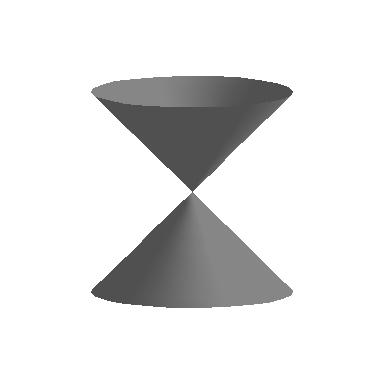
\includegraphics[width=2in]{./ConicsGraphics/cone.jpg}}

If we slice the cone with a horizontal plane the resulting curve is a \index{circle ! from slicing a cone} \textbf{circle}.

\begin{center}

\begin{tabular}{cc}

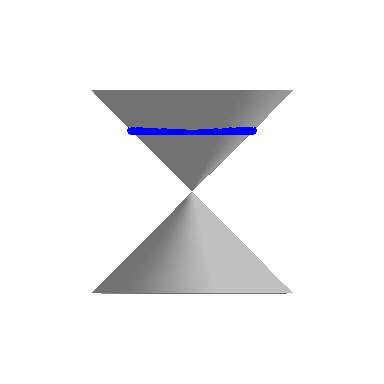
\includegraphics[width=2in]{./ConicsGraphics/Circle01.jpg} & 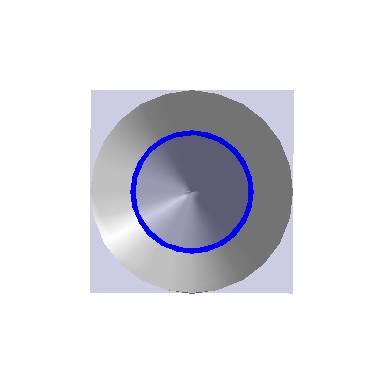
\includegraphics[width=2in]{./ConicsGraphics/Circle02.jpg} \\

\end{tabular}

\end{center}

\pagebreak

Tilting the plane ever so slightly produces an \index{ellipse ! from slicing a cone} \textbf{ellipse}.

\begin{center}

\begin{tabular}{cc}

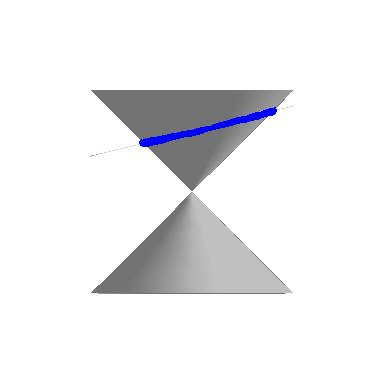
\includegraphics[width=2in]{./ConicsGraphics/Ellipse01.jpg} & 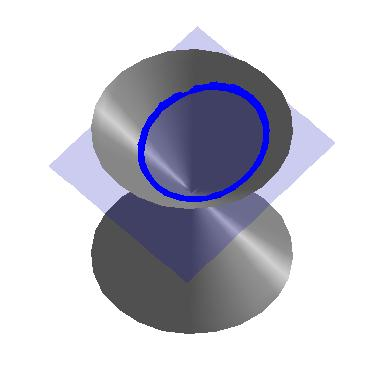
\includegraphics[width=2in]{./ConicsGraphics/Ellipse02.jpg} \\

\end{tabular}

\end{center}

If the plane cuts parallel to the cone, we get a \index{parabola ! from slicing a cone} \textbf{parabola}.

\begin{center}

\begin{tabular}{cc}

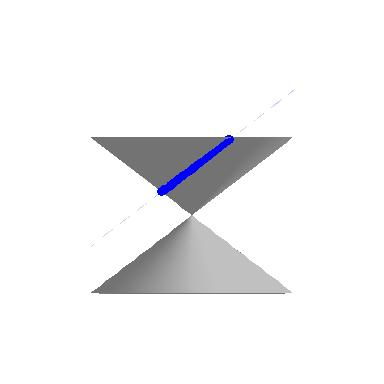
\includegraphics[width=2in]{./ConicsGraphics/Parabola01.jpg} & 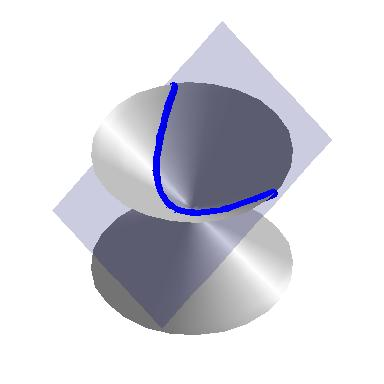
\includegraphics[width=2in]{./ConicsGraphics/Parabola02.jpg} \\

\end{tabular}

\end{center}

If we slice the cone with a vertical plane, we get a \index{hyperbola ! from slicing a cone} \textbf{hyperbola}.

\begin{center}

\begin{tabular}{cc}

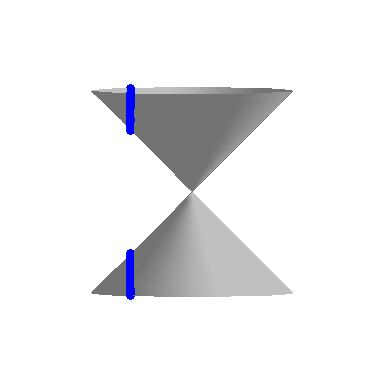
\includegraphics[width=2in]{./ConicsGraphics/Hyperbola01.jpg} & 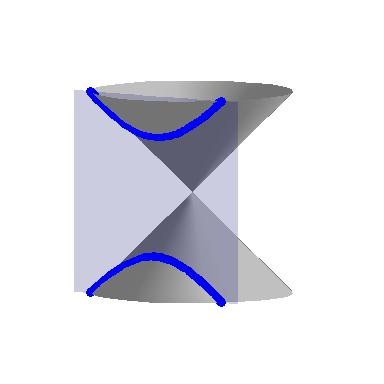
\includegraphics[width=2in]{./ConicsGraphics/Hyperbola02.jpg} \\

\end{tabular}

\end{center}

For a wonderful animation describing the conics as intersections of planes and cones, see Dr. Louis Talman's  \href{http://clem.mscd.edu/~talmanl/HTML/ConicSections.html}{\underline{Mathematics Animated Website}}.

If the slicing plane contains the vertex of the cone, we get the so-called `degenerate' conics:  a point, a line, or two intersecting lines.  


\begin{center}

\begin{tabular}{cc}

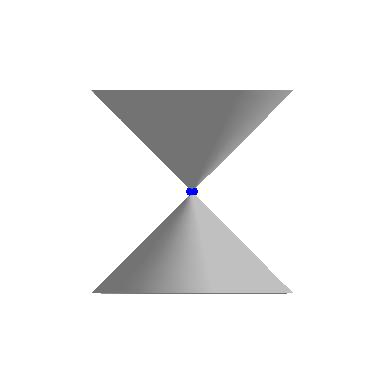
\includegraphics[width=2in]{./ConicsGraphics/Point01.jpg} & 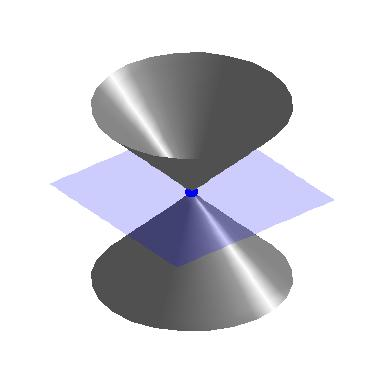
\includegraphics[width=2in]{./ConicsGraphics/Point02.jpg} \\


\includegraphics[width=2in]{./ConicsGraphics/Ilines01.jpg} & 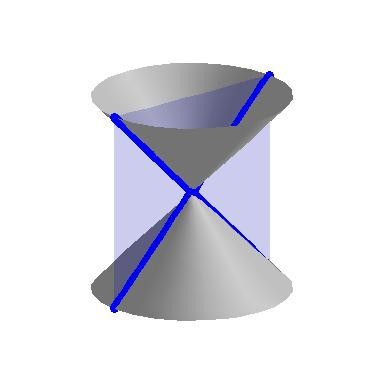
\includegraphics[width=2in]{./ConicsGraphics/Ilines02.jpg}\\

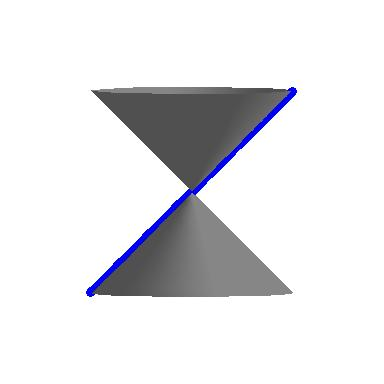
\includegraphics[width=2in]{./ConicsGraphics/Tline01.jpg} & 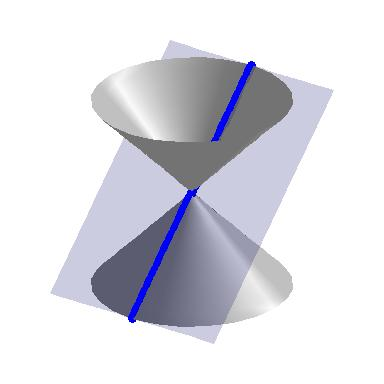
\includegraphics[width=2in]{./ConicsGraphics/Tline02.jpg} \\

\end{tabular}

\end{center}


We will focus the discussion on the non-degenerate cases: circles, parabolas, ellipses, and hyperbolas, in that order. It's not necessary to memorize the description of each conic section. We'd just like you to understand that each conic section is the graph of an equation which can be rearranged into a certain \emph{standard equation}. This standard equation is useful, because it allows us to say something about various geometric properties of the graph. In addition, we will only discuss conic sections centered at the origin.
\newpage

%\typeout{************************************************}
%\typeout{Circles}
%\typeout{************************************************}
\section{Circles}
Recall from Geometry that a circle can be determined by fixing a point (called the \emph{center}) and a positive number (called the \emph{radius}) as follows. \index{circle ! radius of} \index{circle ! center of} \index{center ! of a circle} \index{radius ! of a circle}

\begin{definition}
A \index{circle ! definition of}\dfn{circle} with center $(h,k)$ and radius $r > 0$ is the set of all points $(x, y)$ in the plane whose distance to $(h,k)$ is $r$. 
\end{definition} 

\begin{image}
  \begin{tikzpicture}
    \begin{axis}[axis equal image, ticks=none,axis y line=none, axis x line=none]
       
	\draw (axis cs:0, 0) circle [color=penColor, x radius=6, y radius=6,very thick];
	\addplot[penColor, mark=x, only marks] coordinates {(0,0)};
	\node[above] (center) at (axis cs:0, 0) {$(h, k)$};
	\draw[<->, dashed] (axis cs:0, 0) -- (axis cs: 3, -5.196);
	\addplot[penColor, mark=o, only marks] coordinates {(3, -5.196)};	
	\node[right] (point) at (axis cs: 3, -5.4) {$(x, y)$};
	\node[left] (radius) at (axis cs: 1.5, -2.5) {$r$};

    \end{axis}
  \end{tikzpicture}
\end{image}

We  express this relationship algebraically using the Distance Formula as 
\[r = \sqrt{(x - h)^2 + (y-k)^2}\]  
By squaring both sides of this equation, we get an equivalent equation (since $r > 0$) which gives us the standard equation of a circle.

\begin{definition} \index{circle ! standard equation} \dfn{The standard equation of a circle} with center $(h,k)$ and radius $r >0$ is $(x-h)^2 + (y-k)^2 = r^2.$
\end{definition}

This is the first example of a standard equation. If we are given a standard equation of a circle, we can easily find its center and its radius, which is all that we need to be able to draw the circle in the $xy$-plane. In other courses, we would spend a lot of time taking an equation, converting it into a standard equation, recognizing it as the standard equation of a conic section, and then using the information provided by the standard equation to graph the relation. For our purposes, we only need to know that this process can be done. 

We close this section with the most important circle in all of mathematics:  the \emph{unit circle}.

\begin{definition}
\label{UnitCircle}
The \dfn{unit circle} \index{unit circle ! definition of} is the circle centered at $(0,0)$ with a radius of $1$.  The standard equation of the unit circle is $x^2 + y^2 = 1.$

\end{definition}

As you will soon see, the unit circle is central to the study of trigonometry.

%\typeout{************************************************}
%\typeout{Parabolas}
%\typeout{************************************************}
\section{Parabolas}
We know that parabolas are the graphs of quadratic functions. To our surprise and delight, we may also define parabolas in terms of distance.

\begin{definition}
Let $F$ be a point in the plane and $D$ be a line not containing $F$.   A \index{parabola ! definition of}  \dfn{parabola} is the set of all points equidistant from $F$ and $D$.  The point $F$ is called the \dfn{focus} \index{parabola ! focus} \index{focus (foci) ! of a parabola} of the parabola and the line $D$ is called the \dfn{directrix} \index{parabola ! directrix} \index{directrix ! of a parabola} of the parabola. The \index{parabola ! vertex} \index{vertex ! of a parabola} \dfn{vertex} is the point on the parabola closest to the focus.  
\end{definition}

\begin{image}
  \begin{tikzpicture}
    \begin{axis}[axis equal image, ticks=none,axis y line=none,axis x line=none]
       
	\addplot[<->,domain=-7:7, very thick] {.125*x^2};
	\addplot[<->, domain=-7:7, thick] {-2};
	\node[below] (directrix) at (axis cs: 6, -2) {$D$};

	%points on parabola
	\addplot[penColor, mark=o, only marks] coordinates {(0,0)};
	\node[below] (vertex) at (axis cs: 0.5, 0) {$V$};
	\addplot[penColor, mark=o, only marks] coordinates {(2,0.5)};
	\addplot[penColor, mark=o, only marks] coordinates {(-2,0.5)};
	\addplot[penColor, mark=o, only marks] coordinates {(4,2)};
	\addplot[penColor, mark=o, only marks] coordinates {(-4,2)};
	\addplot[penColor, mark=o, only marks] coordinates {(6,4.5)};
	\addplot[penColor, mark=o, only marks] coordinates {(-6,4.5)};
	
	%focus
	\addplot[penColor, mark=*, only marks] coordinates {(0,2)};
	\node[above] (focus) at (axis cs: 0,2) {$F$};

	% lines from focus to parabola
	\draw[dashed] (axis cs:0, 2) -- (axis cs: 0,0);
	\draw[dashed] (axis cs:0, 2) -- (axis cs: 2, 0.5);
	\draw[dashed] (axis cs:0, 2) -- (axis cs: -2,0.5);
	\draw[dashed] (axis cs:0, 2) -- (axis cs: 4,2);
	\draw[dashed] (axis cs:0, 2) -- (axis cs: -4,2);
	\draw[dashed] (axis cs:0, 2) -- (axis cs: 6,4.5);
	\draw[dashed] (axis cs:0, 2) -- (axis cs: -6,4.5);

	% lines from parabola to directrix
	\draw[dashed] (axis cs:0, -2) -- (axis cs: 0,0);
	\draw[dashed] (axis cs:2, -2) -- (axis cs: 2, 0.5);
	\draw[dashed] (axis cs:-2, -2) -- (axis cs: -2,0.5);
	\draw[dashed] (axis cs:4, -2) -- (axis cs: 4,2);
	\draw[dashed] (axis cs:-4, -2) -- (axis cs: -4,2);
	\draw[dashed] (axis cs:6, -2) -- (axis cs: 6,4.5);
	\draw[dashed] (axis cs:-6, -2) -- (axis cs: -6,4.5);
    \end{axis}
  \end{tikzpicture}
\end{image}

Each dashed line from the point $F$ to a point on the curve has the same length as the dashed line from the point on the curve to the line $D$.  The point suggestively labeled $V$ is, as you should expect, the vertex. Notice that the focus $F$ is not actually a point on the parabola, but only serves to help in its construction.

As with circles, there is a standard equation for parabolas.   
\begin{definition} \index{parabola ! standard equation ! vertical} The \dfn{standard equation of a parabola} which opens up or down with vertex $(h,k)$ and focal length $|p|$ is

\[ (x-h)^2 = 4p(y-k) \]

If $p>0$, the parabola opens upwards;  if $p < 0$, it opens downwards. The \dfn{focal length} of the parabola is the distance from the focus to the vertex. 
\end{definition}

Notice that in the standard equation of the parabola above, only one of the variables, $x$, is squared. This is a quick way to distinguish an equation of a parabola from that of a circle because in the equation of a circle, both variables are squared.

Recall from our earlier discussion of inverse functions that interchanging the roles of $x$ and $y$ results in reflecting the graph across the line $y = x$. Therefore, if we interchange the roles of $x$ and $y$, we can produce `horizontal' parabolas: parabolas which open to the left or to the right. The directrices (plural of `directrix') of such animals would be vertical lines and the focus would either lie to the left or to the right of the vertex, as seen below.

\begin{image}
  \begin{tikzpicture}
    \begin{axis}[axis equal image, ticks=none,axis y line=none,axis x line=none]
       
	\addplot[->,domain=0:6, very thick] {sqrt(8*x)};
	\addplot[->,domain=0:6, very thick] {-sqrt(8*x)};
	\draw[<->, thick] (axis cs:-2, 7) -- (axis cs: -2, -7);
	\node[left] (directrix) at (axis cs: -2, 6) {$D$};

	%vertex
	\node[left] (vertex) at (axis cs: 0,0) {$V$};
	\addplot[penColor, mark=o, only marks] coordinates {(0,0)};
	
	%focus
	\addplot[penColor, mark=*, only marks] coordinates {(2,0)};
	\node[right] (focus) at (axis cs: 2, 0) {$F$};

	
    \end{axis}
  \end{tikzpicture}
\end{image}

\begin{definition}
\index{parabola ! standard equation ! horizontal} \dfn{The standard equation of a parabola} that opens to the left or right with vertex $(h,k)$ and focal length $|p|$ is

\[ (y-k)^2 = 4p(x-h) \]

If $p>0$, the parabola opens to the right;  if $p < 0$, it opens to the left.
\end{definition}

%\typeout{************************************************}
%\typeout{Ellipses}
%\typeout{************************************************}
\section{Ellipses}
In the definition of a circle, we fixed a point called the \emph{center} and considered all of the points which were a fixed distance $r$ from that one point.  For our next conic section, the ellipse, we fix two distinct points and a distance $d$ to use in our definition.  

\begin{definition}
Given two distinct points $F_{1}$ and $F_{2}$ in the plane and a fixed distance $d$, an \index{ellipse ! definition of}  \dfn{ellipse} is the set of all points $(x, y)$ in the plane such that the sum of each of the distances from $F_{1}$ and $F_{2}$ to $(x, y)$ is $d$.  The points $F_{1}$ and $F_{2}$ are called the \index{ellipse ! foci} \index{focus (foci) ! of an ellipse} \dfn{foci} (the plural of `focus') of the ellipse.
\end{definition}

In the figure below, $d_1$ is the distance from $(x, y)$ to $F_1$, and $d_2$ is the distance from $(x, y)$ to $F_2$. Since $(x, y)$ is on the ellipse, $d_1 + d_2 = d$ for some fixed $d$. 
\begin{image}
  \begin{tikzpicture}
    \begin{axis}[axis equal image, ticks=none,axis y line=none, axis x line=none]
       
	\draw (axis cs:0, 0) circle [color=penColor, x radius=5, y radius=4,very thick];
	\draw[dashed] (axis cs:3, 0) -- (axis cs: 4,2.4);
	\node (d1) at (axis cs: -1, 1.1) {$d_1$};
	\node (d2) at (axis cs: 3, 1.1) {$d_2$};
	\draw[dashed] (axis cs:-3, 0) -- (axis cs: 4,2.4);
	\addplot[penColor, mark=*, only marks] coordinates {(3,0)};	
	\addplot[penColor, mark=*, only marks] coordinates {(-3,0)};
	\addplot[penColor, mark=o, only marks] coordinates {(4, 2.4)};
	\node[below] (f1) at (axis cs: -3, 0) {$F_1$};
	\node[below] (f2) at (axis cs: 3, 0) {$F_2$};
	\node[right] (point) at (axis cs: 4,2.4) {$(x, y)$};

    \end{axis}
  \end{tikzpicture}
\end{image}


We may imagine taking a length of string and anchoring it to two points on a piece of paper.  The curve traced out by taking a pencil and moving it so the string is always taut is an ellipse. Notice again that the foci are not actually points on the ellipse, but only serve to help in its construction.

The \index{ellipse ! center} \index{center ! of an ellipse} \emph {center} of the ellipse is the midpoint of the line segment connecting the two foci.  The \index{ellipse ! major axis} \index{major axis of an ellipse} \emph{major axis} of the ellipse is the line segment connecting two opposite ends of the ellipse which also contains the center and foci.  The \index{ellipse ! minor axis} \index{minor axis of an ellipse} \emph{minor axis} of the ellipse is the line segment connecting two opposite ends of the ellipse which contains the center but is perpendicular to the major axis. The major axis is always the longer of the two segments. The \index{ellipse ! vertices} \index{vertex ! of an ellipse} \emph {vertices} of an ellipse are the points of the ellipse which lie on the major axis.  Notice that the center is also the midpoint of the major axis, hence it is the midpoint of the vertices.  In pictures we have,

\begin{image}
  \begin{tikzpicture}
    \begin{axis}[axis equal image, ticks=none,axis y line=none, axis x line=none]
       
	\draw (axis cs:0, 0) circle [color=penColor, x radius=5, y radius=4,very thick];
	\addplot[penColor, mark=*, only marks] coordinates {(3,0)};	
	\addplot[penColor, mark=*, only marks] coordinates {(-3,0)};
	\addplot[penColor, mark=x, only marks] coordinates {(0,0)};
	\addplot[penColor, mark=o, only marks] coordinates {(-5,0)};
	\addplot[penColor, mark=o, only marks] coordinates {(5,0)};
	\node[below] (f1) at (axis cs: -3, 0) {$F_1$};
	\node[below] (f2) at (axis cs: 3, 0) {$F_2$};
	\node[left] (v1) at (axis cs: -5, 0) {$V_1$};
	\node[right] (v2) at (axis cs: 5, 0) {$V_2$};
	\node[below] (c) at (axis cs: 0, 0) {$C$};
	\draw[dotted] (axis cs:-5, 0) -- (axis cs: 5,0);
	\draw[dotted] (axis cs:0,-4) -- (c) -- (axis cs: 0,4);
	\node (maj) at (axis cs:2.5, 0.5) {\tiny Major Axis};
	\node (min) at (axis cs:-0.5,2) {\tiny \rotatebox{90}{Minor Axis}};

    \end{axis}
  \end{tikzpicture}
\end{image}

There is also a standard equation for ellipses. 
\begin{definition}
\index{ellipse ! standard equation} For positive unequal numbers $a$ and $b$, \dfn{the standard equation of an ellipse} with center $(h,k)$ is

\[ \dfrac{(x-h)^2}{a^2} + \dfrac{(y-k)^2}{b^2} = 1 \]
\end{definition}

First note that the values $a$ and $b$ determine how far in the $x$ and $y$ directions, respectively, one counts from the center to arrive at points on the ellipse.  Also take note that if $a > b$, then we have an ellipse whose major axis is horizontal, and hence, the foci lie to the left and right of the center.  In this case, the distance from the center to the focus, $c$, can be found by $c = \sqrt{a^2 - b^2}$.  If $b > a$, the roles of the major and minor axes are reversed, and the foci lie above and below the center. In this case, $c = \sqrt{b^2 - a^2}$.  In either case, $c$ is the distance from the center to each focus, and $c = \sqrt{\mbox{bigger denominator} - \mbox{smaller denominator}}$.   Finally, it is worth mentioning that if we take the standard equation of a circle and divide both sides by $r^2$, we get

\begin{definition} \index{circle ! standard equation, alternate} \dfn{The alternate standard equation of a circle} with center $(h,k)$ and radius $r >0$ is

\[ \dfrac{(x-h)^2}{r^2} + \dfrac{(y-k)^2}{r^2} = 1 \]

\end{definition}
  
Notice the similarity between the two equations. Both involve a sum of squares equal to $1$;  the difference is that with a circle, the denominators are the same, and with an ellipse, they are different.  If we take a transformational approach, we can consider both equations as shifts and stretches of the unit circle $x^2 + y^2 = 1$.  Replacing $x$ with $(x-h)$ and $y$ with $(y-k)$ causes the usual horizontal and vertical shifts.  Replacing $x$ with $\frac{x}{a}$ and $y$ with $\frac{y}{b}$ causes the usual vertical and horizontal stretches.  In other words, it is perfectly fine to think of an ellipse as the deformation of a circle in which the circle is stretched farther in one direction than the other.

%\typeout{************************************************}
%\typeout{Hyperbolas}
%\typeout{************************************************}
\section{Hyperbolas}
In the definition of an ellipse, we fixed two points called foci and looked at points whose distances to the foci always \emph{added} to a constant distance $d$.  Those prone to syntactical tinkering may wonder what, if any, curve we'd generate if we replaced \emph{added} with \emph{subtracted}.  The answer is a hyperbola.

\begin{definition}
Given two distinct points $F_{1}$ and $F_{2}$ in the plane and a fixed distance $d$, a \index{hyperbola ! definition of}  \dfn{hyperbola} is the set of all points $(x, y)$ in the plane such that the difference of each of the distances from $F_{1}$ and $F_{2}$ to $(x, y)$ is $d$.  The points $F_{1}$ and $F_{2}$ are called the \index{hyperbola ! foci} \index{focus (foci) ! of an hyperbola}\dfn{foci} of the hyperbola.
\end{definition}

\begin{image}
  \begin{tikzpicture}
    \begin{axis}[axis equal image, ticks=none,axis y line=none, axis x line=none]
	\coordinate (center) at (axis cs:0, 0);
	\tikzhyperbola[color=penColor2, <->]{0}{(center)}{300}{400}{60};

	%foci
	\addplot[penColor, mark=*, only marks] coordinates {(-5,0)};
	\addplot[penColor, mark=*, only marks] coordinates {(5,0)};
	\node[below] (f1) at (axis cs: -5, 0) {$F_1$};
	\node[below] (f2) at (axis cs: 5, 0) {$F_2$};

	%points
	\addplot[penColor, mark=o, only marks] coordinates {(3.5,2.4)};
	\addplot[penColor, mark=o, only marks] coordinates {(-3.25,-1.667)};
	\node[below] (p2) at (axis cs: -2.05,-2.25) {$(x_2, y_2)$};
	\node[below] (p1) at (axis cs: 4.95,2.5) {$(x_1, y_1)$};

	%segments
	\draw[dashed] (axis cs: 5, 0) -- (axis cs: 3.5,2.4) -- (axis cs: -5, 0);
	\draw[dashed] (axis cs: -5, 0) -- (axis cs: (-3.25,-1.667) -- (axis cs: 5, 0);
	
    \end{axis}
  \end{tikzpicture}
\end{image}

In the figure above:

\[ \begin{array}{rclr} \mbox{the distance from $F_{\mbox{\tiny$1$}}$ to $(x_{\mbox{\tiny$1$}}, y_{\mbox{\tiny$1$}})$} - \mbox{the distance from $F_{\mbox{\tiny$2$}}$ to $(x_{\mbox{\tiny$1$}}, y_{\mbox{\tiny$1$}})$} & = & d & \\ \end{array}\]

and

\[ \begin{array}{rclr} \mbox{the distance from $F_{\mbox{\tiny$2$}}$ to $(x_{\mbox{\tiny$2$}}, y_{\mbox{\tiny$2$}})$} - \mbox{the distance from $F_{\mbox{\tiny$1$}}$ to $(x_{\mbox{\tiny$2$}}, y_{\mbox{\tiny$2$}})$} & = & d & \\ \end{array}\]

Note that the hyperbola has two parts, called \index{hyperbola ! branch} \emph{branches}.  The \index{hyperbola ! center}\index{center ! of a hyperbola}\emph{center} of the hyperbola is the midpoint of the line segment connecting the two foci.  The \index{hyperbola ! transverse axis}\index{transverse axis of a hyperbola}\emph{transverse axis} of the hyperbola is the line segment connecting two opposite ends of the hyperbola which also contains the center and foci.  The \index{hyperbola ! vertices}\index{vertex ! of a hyperbola}\emph{vertices} of a hyperbola are the points of the hyperbola which lie on the transverse axis.  In addition, there are lines called \index{hyperbola ! asymptotes}\index{asymptote ! of a hyperbola}\emph{asymptotes} which the branches of the hyperbola approach for large $x$ and $y$ values.   They serve as guides to the graph.  In pictures,

\begin{image}
  \begin{tikzpicture}
    \begin{axis}[axis equal image, ticks=none,axis y line=none, axis x line=none]
	\coordinate (center) at (axis cs:0, 0);
	\tikzhyperbola[color=penColor2, <->]{0}{(center)}{300}{400}{60};

	%foci
	\addplot[penColor, mark=*, only marks] coordinates {(-5,0)};
	\addplot[penColor, mark=*, only marks] coordinates {(5,0)};
	\node[below] (f1) at (axis cs: -5, 0) {$F_1$};
	\node[below] (f2) at (axis cs: 5, 0) {$F_2$};

	%center
	\addplot[penColor, mark=x, only marks] coordinates {(0,0)};
	\node[below] (c) at (axis cs: 0, -0.2) {$C$};

	%vertices
	\addplot[penColor, mark=o, only marks] coordinates {(3,0)};
	\addplot[penColor, mark=o, only marks] coordinates {(-3,0)};
	\node[right] (v2) at (axis cs: 3,0) {$V_2$};
	\node[left] (v1) at (axis cs: -3,0) {$V_1$};

	%segments
	\draw[dotted] (axis cs: -3, 0) -- (axis cs: 3, 0);
	\node (tv) at (axis cs:0, 0.5) {\tiny Transverse Axis};

	%asymptotes
	\addplot[dashed, <-, domain=-5:0]{4*x/3} node{};
	\addplot[dashed, ->, domain=0.5:5]{4*x/3} node{};
	\addplot[dashed, <-, domain=-5:-0.5]{(-4)*x/3} node{};
	\addplot[dashed, ->, domain=0:5]{(-4)*x/3} node{};
    \end{axis}
  \end{tikzpicture}
\end{image}

The above hyperbola has center $C$, foci $F_1$ and $F_2$, and vertices $V_1$ and $V_2$. The asymptotes are represented by dashed lines.


The \index{hyperbola ! conjugate axis}\index{conjugate axis of a hyperbola}\emph{conjugate axis} of a hyperbola is the line segment through the center which is perpendicular to the transverse axis and has the same length as the line segment through a vertex which connects the asymptotes.

As with all the other conic sections, we have a standard equation for hyperbolas.

\begin{definition} \index{hyperbola ! standard equation ! horizontal}  For positive numbers $a$ and $b$, \dfn{the equation of a hyperbola} opening left and right with center $(h,k)$ is

\[ \dfrac{(x-h)^2}{a^2} - \dfrac{(y-k)^2}{b^2} = 1 \]

\end{definition}
  
If the roles of $x$ and $y$ were interchanged, then the hyperbola's branches would open upwards and downwards and we would get a `vertical' hyperbola.

\begin{definition} \index{hyperbola ! standard equation ! vertical} For positive numbers $a$ and $b$, \dfn{the equation of a hyperbola} opening upwards and downwards with center $(h,k)$ is

\[ \dfrac{(y-k)^2}{b^2} - \dfrac{(x-h)^2}{a^2} = 1 \]

\end{definition}
The values of $a$ and $b$ determine how far in the $x$ and $y$ directions, respectively, one counts from the center to determine the rectangle through which the asymptotes pass.  In both cases, the distance from the center to the foci, $c$, can be found by the formula $c = \sqrt{a^2 + b^2}$.  Lastly, note that we can quickly distinguish the equation of a hyperbola from that of a circle or ellipse because the hyperbola formula involves a \emph{difference} of squares where the circle and ellipse formulas both involve the \emph{sum} of squares.

\end{document}
